\documentclass[12pt, twoside]{article}
\usepackage[letterpaper, margin=1in, headsep=0.5in]{geometry}
\usepackage[english]{babel}
\usepackage[utf8]{inputenc}
\usepackage{amsmath}
\usepackage{amsfonts}
\usepackage{amssymb}
\usepackage{tikz}
\usetikzlibrary{quotes, angles}
\usepackage{graphicx}
\usepackage{enumitem}
\usepackage{multicol}

\newif\ifmeta
\metatrue %print standards and topics tags

\title{Regents Geometry}
\author{Chris Huson}
\date{September 2020}

\usepackage{fancyhdr}
\pagestyle{fancy}
\fancyhf{}
\renewcommand{\headrulewidth}{0pt} % disable the underline of the header
\raggedbottom


\fancyhead[LE]{\thepage}
\fancyhead[RO]{\thepage \\ Name: \hspace{4cm} \,\\}
\fancyhead[L]{BECA / Dr. Huson / Geometry 05-Transformations\\* pset ID: 67}

\begin{document}

\subsubsection*{5-8DN-similarity-ratios}
\begin{enumerate}
\item Triangle $ABC$ is dilated with a factor of $\frac{3}{2}$ centered at $A$, yielding $\triangle ADE$, as shown. Given $AB=10$, $BC=12$, and $AC=14$. \\[0.25cm] Find $AD$, $AE$, and $DE$.
    \begin{flushright}
        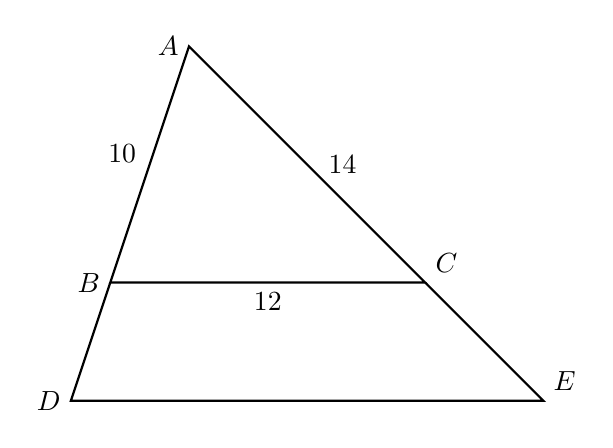
\begin{tikzpicture}[scale=0.5]
          \draw [thick]
          (0,0)node[left]{$B$}--
          (8,0)node[above right]{$C$}--
          (2,6)node[left]{$A$}--cycle;
          \draw [thick]
          (0,0)--
          (-1,-3)node[left]{$D$}--
          (11,-3)node[above right]{$E$}--(8,0);
          \node at (4,0)[below]{$12$};
          \node at (5.3, 3)[right]{$14$};
          \node at (0.3, 2.8)[above]{$10$};
        \end{tikzpicture}
      \end{flushright}

   \vspace{2cm}

\item Given $\triangle ABP \sim \triangle JKP$ as shown below. $\overline{AB} \parallel \overline{JK}$. $AP=5.7$, $JP=11.4$, and $JK=14.8$. Find $AB$.
    \begin{flushright}
      \begin{tikzpicture}[scale=1.4]
          \draw [thick]
            (0.25,-1)node[right]{$B$}--
            (-0.5,2)node[left]{$K$}--
            (4,0)node[right]{$J$}--
            (0,0)node[above right]{$P$}--
            (-2,0)node[left]{$A$}--cycle;
        \end{tikzpicture}
       \end{flushright}
       \vspace{2cm}

\item Find the image of $A(-3,1)$ after the translation $(x,y) \rightarrow (x+4,y-2)$.
  
\newpage
\item The vertices of $\triangle JKL$ have the coordinates $J(-4,-2)$, $K(-1,-1)$, and $L(-2,3)$, as shown below. \\[0.5cm]
    Apply a translation of $(x,y) \rightarrow (x+7, y+2)$ to $\triangle JKL$  yielding the triangle $\triangle J'K'L'$. List its coordinates in a table and plot it on the set of axes below, labeling the vertices.
    \begin{flushright}
      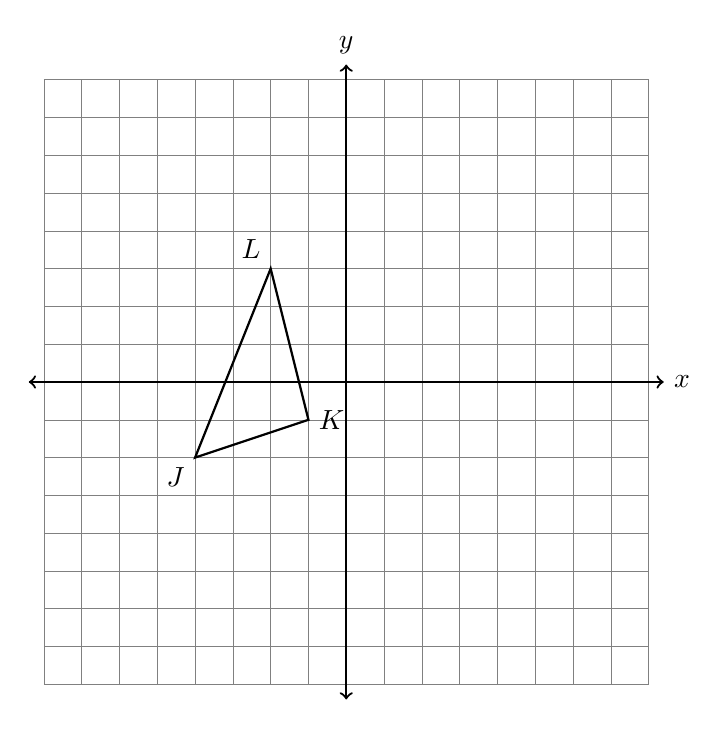
\begin{tikzpicture}[scale=.48]
        \draw [help lines] (-8,-8) grid (8,8);
        \draw [thick, <->] (-8.4,0) -- (8.4,0) node [right] {$x$};
        \draw [thick, <->] (0,-8.4)--(0,8.4) node [above] {$y$};

        \draw [thick]
        (-4,-2) node[below left] {$J$}--
        (-1,-1) node[right] {$K$}--
        (-2,3) node[above left] {$L$}--
        cycle;
      \end{tikzpicture}
    \end{flushright}

\item A rotation of $90^\circ$ is applied to $\triangle ABC$, mapping it onto $\triangle PQR$, as shown.  \\[0.25cm]
 Which triangle has the larger area, or are they equal? Justify your answer.\\
     \begin{tikzpicture}[scale=.48]
       \draw [thick, <->] (-7.4,0) -- (10.4,0) node [right] {$x$};
       \draw [thick, <->] (0,-5.4)--(0,10.4) node [above] {$y$};
       \draw [thick]
       (4,-2) node[below left] {$A$}--
       (8,2) node[right] {$B$}--
       (1,1) node[above right] {$C$}--cycle;
       \draw [thick]
       (2,4) node[right] {$P$}--
       (-2,8) node[above] {$Q$}--
       (-1,1) node[below left] {$R$}--cycle;
     \end{tikzpicture}

\newpage
\item Triangle $ADE$ and its midline $\overline{BC}$ are drawn, with $B$ the midpoint of $\overline{AD}$ and $C$ the midpoint of $\overline{AE}$. The two medians $\overline{AE}$ and $\overline{AE}$ are drawn, as shown, intersecting in point $F$, the centroid.\\[0.25cm]
  $\triangle FCB \sim \triangle FDE$ with scale factor $k=2$.\\[0.25cm]
  Given $BC=7$, find $DE$. \\[0.25cm] Given $BF=4$, find $FE$. %\vspace{1cm}
  \begin{flushright}
      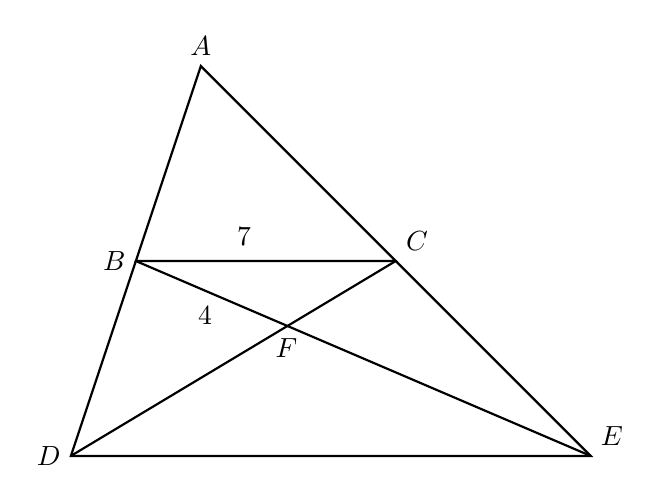
\begin{tikzpicture}[scale=0.55]
        \draw [thick]
        (0.5,1.5)node[left]{$B$}--
        (6.5,1.5)node[above right]{$C$}--
        (2,6)node[above]{$A$}--cycle;
        \draw [thick]
        (0.5,1.5)--
        (-1,-3)node[left]{$D$}--
        (11,-3)node[above right]{$E$}--(6.5,1.5);
        \draw [thick] (0.5,1.5)--(11,-3);
        \draw [thick] (6.5,1.5)--(-1,-3);
        \node at (3,2.5)[below]{$7$};
        \node at (3.5, -0.5)[right]{$F$};
        \node at (2.1, -0.2)[above]{$4$};
        %\node at (-0.7, -1)[above]{$5$};
      \end{tikzpicture}
    \end{flushright} \vspace{1cm}

\item The trapezoid $ABCD$, shown below, undergoes a rigid transformation carrying it onto trapezoid $WXYZ$. State the transformation. (be specific)\\
    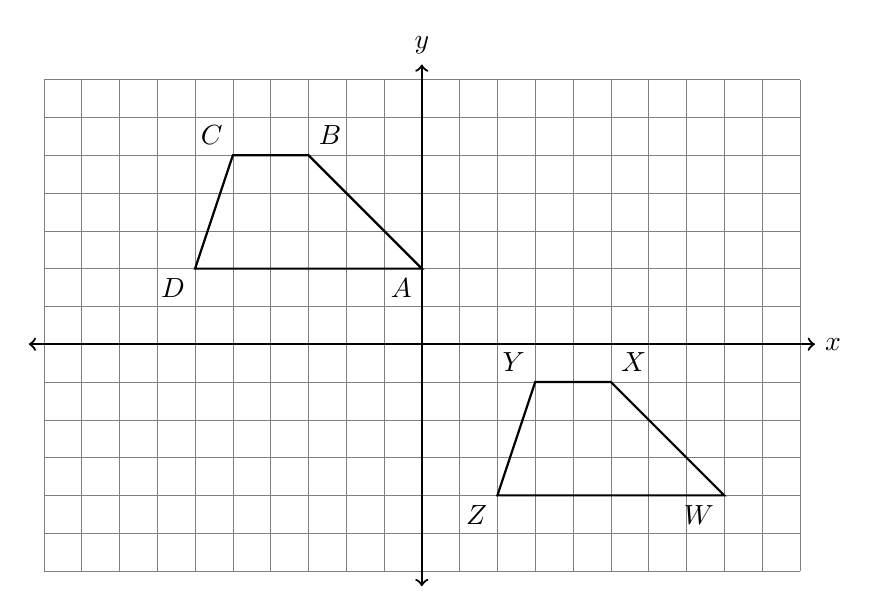
\begin{tikzpicture}[scale=.48]
      \draw [help lines] (-10,-6) grid (10,7);
      \draw [thick, <->] (-10.4,0) -- (10.4,0) node [right] {$x$};
      \draw [thick, <->] (0,-6.4)--(0,7.4) node [above] {$y$};
      \draw [thick]
        (2,-4) node[below left] {$Z$}--
        (3,-1) node[above left] {$Y$}--
        (5,-1) node[above right] {$X$}--
        (8,-4) node[below left] {$W$}--cycle;
      \draw [thick]
        (0,2) node[below left] {$A$}--
        (-3,5) node[above right] {$B$}--
        (-5,5) node[above left] {$C$}--
        (-6,2) node[below left] {$D$}--cycle;
    \end{tikzpicture}

\newpage
\item Apply a rotation of $90^\circ$ counterclockwise to $\triangle ZAP$. Plot and label $\triangle Z'A'P'$ on the axes below and make a table listing its coordinates.
    \begin{flushright}
      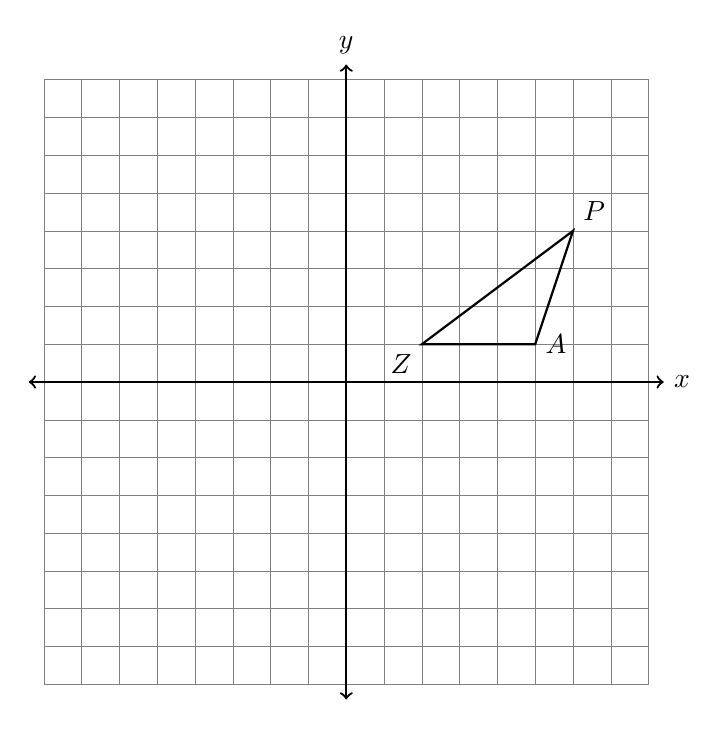
\begin{tikzpicture}[scale=.48]
        \draw [help lines] (-8,-8) grid (8,8);
        \draw [thick, <->] (-8.4,0) -- (8.4,0) node [right] {$x$};
        \draw [thick, <->] (0,-8.4)--(0,8.4) node [above] {$y$};
        \draw [thick]
          (2,1) node[below left] {$Z$}--
          (5,1) node[right] {$A$}--
          (6,4) node[above right] {$P$}--cycle;
      \end{tikzpicture}
    \end{flushright}

\item In  $\triangle ABC$ shown below, $m\angle A=(3x+13)^\circ$, $m\angle B=(4x+4)^\circ$, and $m\angle C=(2x-8)^\circ$. What is $m\angle A$?
    \begin{flushright}
        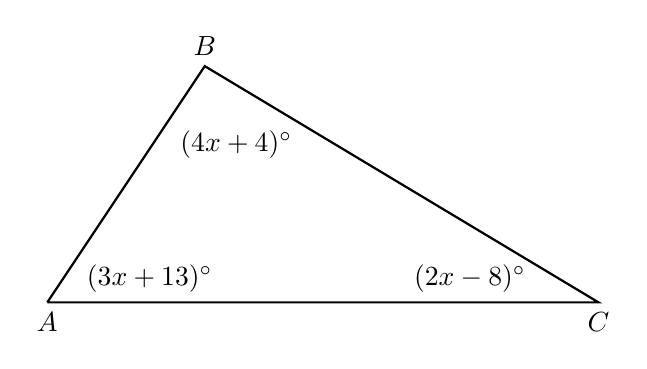
\begin{tikzpicture}
          \draw [thick]
            (2,0)node[below]{$A$}--
            (9,0)node[below]{$C$}--
            (4,3)node[above]{$B$} --(2,0);
            \node at (3.3,0)[above]{$(3x+13)^\circ$};
            \node at (8.2,0)[above left]{$(2x-8)^\circ$};
            \node at (4.4,2.3)[below]{$(4x+4)^\circ$};
        \end{tikzpicture}
      \end{flushright}

\end{enumerate}
\end{document}